\documentclass{beamer}
%\usepackage{beamerthemeBerkeley}
% Use either the one above or the one below
\usetheme{default}

\usepackage{amsmath,amssymb,amsthm,multirow,algorithmic,graphics,color,ifpdf}
\usepackage{algorithmic,graphicx,tikz,pgflibraryarrows,pgflibraryplotmarks,pgflibrarysnakes,pgflibraryshapes}
\usepackage[section]{algorithm}
%\usepackage[matrix,arrow]{xypic}
%\usepackage{fullpage}
\newcommand{\C}{\mathbb{C}}
\newcommand{\R}{\mathbb{R}}
\newcommand{\Z}{\mathbb{Z}}
\newcommand{\N}{\mathbb{N}}
\newcommand{\Q}{\mathbb{Q}}
\newcommand{\F}{\mathbb{F}}
\newcommand{\KP}{\textbf{KP}}
\newcommand{\OW}{\textbf{OW-CPA}}
\newcommand{\INDCPA}{{\textbf{IND-CPA}}}
\newcommand{\INDCCA}{{\textbf{IND-CCA}}}
\newcommand{\INDCCATWO}{{\textbf{IND-CCA2}}}
\newcommand{\A}{\mathcal{A}}
\newcommand{\B}{\mathcal{B}}
\newcommand{\D}{\mathcal{D}}
\newcommand{\E}{\mathcal{E}}
\renewcommand{\c}{\mathcal{C}}
\newcommand{\G}{\mathcal{G}}
\newcommand{\I}{\mathfrak{I}}
\renewcommand{\O}{\mathcal{O}}
\newcommand{\p}{\mathfrak{p}}
\renewcommand{\P}{\mathcal{P}}
\newcommand{\iso}{\cong}
\newcommand{\stacksum}[2]{\genfrac{}{}{0pt}{}{{#1}}{{#2}}} %\substack is better
\newcommand{\jacobi}[2]{{\genfrac{(}{)}{}{}{#1}{#2}}}
\newcommand{\ord}{\operatorname{ord}}
\newcommand{\Res}{\operatorname{Res}}
%\renewcommand{\div}{\operatorname{div}}
\newcommand{\ndiv}{\nmid}
\renewcommand{\div}{\mid}
\newcommand{\Div}{\operatorname{div}}
\newcommand{\Pic}{\operatorname{Pic}}
\newcommand{\End}{\operatorname{End}}
\newcommand{\Cl}{\operatorname{Cl}}
\newcommand{\QR}{\operatorname{QR}}
\newcommand{\QNR}{\overline{\operatorname{QR}}}
\newcommand{\<}{\langle}
\renewcommand{\>}{\rangle}
\newcommand{\union}{\cup}
\newcommand{\intersection}{\cap}
\newcommand{\chr}{\operatorname{char}}
\newcommand{\id}{\operatorname{id}}
\newcommand{\Enc}{\operatorname{Encrypt}}
\newcommand{\Dec}{\operatorname{Decrypt}}
\newcommand{\pub}{{\operatorname{pubkey}}}
\newcommand{\priv}{{\operatorname{privkey}}}
\newcommand{\dlog}{{\operatorname{DLOG}}}
\newcommand{\cdh}{{\operatorname{CDH}}}
\newcommand{\ddh}{{\operatorname{DDH}}}
\newcommand{\bdh}{{\operatorname{BDH}}}
\newcommand{\dbdh}{{\operatorname{DBDH}}}
\newcommand{\LSB}{{\operatorname{LSB}}}
\newcommand{\MSB}{{\operatorname{MSB}}}
\newcommand{\Gal}{{\operatorname{Gal}}}
\renewcommand{\Pr}{{\operatorname{Prob}}}
\newcommand{\lcm}{{\operatorname{lcm}}}
\newcommand{\SL}{{\operatorname{SL}}}
\newcommand{\PSL}{{\operatorname{PSL}}}
\newcommand{\GL}{{\operatorname{GL}}}
\newcommand{\Ell}{{\operatorname{Ell}}}
\renewcommand{\a}{{\mathfrak{a}}}
\renewcommand{\b}{{\mathfrak{b}}}
\renewcommand{\L}{{\mathfrak{L}}}
\newcommand{\ignore}[1]{}
\renewcommand{\algorithmicrequire}{\textbf{Given:}}
\newcommand{\st}{\mid}
\newcommand{\eps}{\varepsilon}
\newcommand{\DL}{\operatorname{DL}}
\newcommand{\CDH}{\operatorname{DH}}
\newcommand{\PI}{\operatorname{PI}}
\newcommand{\BDH}{\operatorname{BDH}}
\newcommand{\IDH}{\operatorname{IDH}}
\newcommand{\IBDH}{\operatorname{IBDH}}

\newlength{\algcwidth} \newlength{\algcheight}
\newcommand{\algc}[1]{%
\settowidth{\algcwidth}{#1} \settoheight{\algcheight}{#1}%
\raisebox{1.2\algcheight}[0pt]{%
\makebox[0pt][l]{\hspace{.4\algcwidth}%
\rule{.6\algcwidth}{0.05\algcheight}}}%
{{#1}}}

\newcommand{\includeonlyiflecture}[1]{#1}
\newcommand{\includeonlyifbook}[1]{}

\newcommand{\cyc}[1]{{\langle #1 \rangle}}
\newcommand{\red}[1]{\textcolor{red}{#1}}
\newcommand{\blue}[1]{\textcolor[rgb]{0.24,0.15,0.70}{#1}}
\newcommand{\green}[1]{\textcolor[rgb]{0,0.8,0}{#1}}
\newcommand{\pink}[1]{\textcolor[rgb]{1,0.2,0.6}{#1}}
\newcommand{\orange}[1]{\textcolor[rgb]{1,0.6,0}{#1}}
\newcommand{\purple}[1]{\textcolor[rgb]{0.4,0.2,0.8}{#1}}


\pgfkeys{/triangle/.code=\tikzset{x={(-0.5cm,-0.866cm)},y={(1cm,0cm)}}}

% This command defines a triangle of dots of given height
\newcommand{\dottriangle}[2][\i-\j]{%
  \foreach \i in {0,...,#2} {%
    \foreach \j in {0,...,\i} {%
      \draw(\i,\j) node{#1};%
    }%
  }}

\title{Towards quantum-resistant cryptosystems
from supersingular elliptic curve isogenies}
\author{David Jao and Luca De Feo}
\date{November 30, 2011}
\institute{University of Waterloo}

\begin{document}

\frame{\titlepage}

%\AtBeginSection[]
%{
%  \begin{frame}<beamer>
%    \frametitle{Outline}
%    \tableofcontents[current]
%  \end{frame}
%}


\begin{frame}
\frametitle{Overview}

Motivation:
\begin{itemize}
\item Construct a quantum-resistant (classical) public-key
  cryptosystem based on maps (isogenies) between elliptic curves.
\item Achieve faster performance than previous isogeny-based
  public-key cryptosystems.
\end{itemize}

Results:
\begin{itemize}
\item Under the assumption that computing a particular class of
  isogenies is infeasible on a quantum computer, we produce a
  quantum-resistant public-key cryptosystem.
\item Against fastest known attacks, at the 128-bit security level,
  our scheme is over $1000$ times faster than previous isogeny-based
  public-key cryptosystems.
\end{itemize}

\end{frame}

\section{Isogenies}

\begin{frame}
\frametitle{Isogenies}
\begin{definition}
  Let $E$ and $E'$ be elliptic curves over $F$.
\begin{itemize}
\item An \emph{isogeny}
  $\phi\colon E \to E'$ is a non-constant algebraic morphism
\[
\phi(x,y) = \left(\frac{f_1(x,y)}{g_1(x,y)},\frac{f_2(x,y)}{g_2(x,y)}
\right)
\]
satisfying $\phi(\infty) = \infty$ (equivalently, $\phi(P+Q) =
\phi(P)+\phi(Q)$).
\item The \emph{degree} of an isogeny is its degree as an algebraic
  map.
\item The \emph{endomorphism ring} $\End(E)$ is the set of isogenies
  from $E(\algc{F})$ to itself, together with the constant
  homomorphism. This set forms a ring under pointwise addition and
  composition.
\end{itemize}
\end{definition}
\end{frame}


\begin{frame}
\frametitle{Ordinary and supersingular curves}

\begin{theorem}
Let $E$ be an elliptic curve defined over a finite field.
As a $\Z$-module, $\dim_{\Z} \End(E)$ is equal to either $2$ or $4$.
\end{theorem}

\begin{definition}
An elliptic curve $E$ over a finite field is \emph{supersingular} if
$\dim_{\Z} \End(E) = 4$, and \emph{ordinary} otherwise.
\end{definition}

 Isogenous curves are always either both ordinary, or both supersingular.
\end{frame}

\begin{frame}
\frametitle{The ordinary case}

Let $E$ be an ordinary elliptic curve with
$\End(E) = \O_D$.

\begin{definition}
The set of isomorphism classes of elliptic curves $E/\F_p$ with
$\End(E) = \O_D$ is denoted $\Ell_{p,n}(\O_D)$, where $n = \#E$.
\end{definition}

\begin{theorem}[Waterhouse 1969]
There is a group action $*\colon \Cl(\O_D) \times \Ell_{p,n}(\O_D) \to
\Ell_{p,n}(\O_D)$, defined as follows.
\begin{itemize}
\item Given $\b \in \Cl(\O_D)$, and $E \in \Ell_{p,n}(\O_D)$, let
  $\phi_\b\colon E \to E'$ be the isogeny corresponding to $\b$.
\item Set $\b * E = E'$. 
\end{itemize}
$\Ell_{p,n}(\O_D)$ is a principal homogeneous space for the group
$\Cl(\O_D)$ under this action. In other words, the action is free and
transitive.
\end{theorem}
\end{frame}

\begin{frame}
\frametitle{Isogeny-based cryptography}
\begin{itemize}
\item Cryptosystems based on isogenies have been proposed by
  Couveignes (1996), Rostovtsev and Stolbunov (2006), and Stolbunov
  (2010).

\item Given $\b$ and $E$, computing $\b * E$ is hard, but it can be
  easy if you choose $\b$ to be of the form $\p_1^{e_1} \p_2^{e_2}
  \cdots \p_t^{e_t}$.

\item Given $E$ and $E'$, computing the quotient seems hard, and (as an
  attacker) you may not have the ability to choose $E$ and $E'$.

\item This leads to the design of public key cryptosystems based on
  group actions.
\end{itemize}
\end{frame}

\begin{frame}
\frametitle{Example: Key exchange}
\begin{description}
\item[Public parameters:] $p$, $E \in \Ell_{p,n}(\O_K)$
\item[Key generation:] Choose an ideal $\b = \p_1^{e_1} \p_2^{e_2}
  \cdots \p_t^{e_t}$.
\item[Public key:] $\b * E$
\item[Private key:] $\b$
\end{description}
To generate a shared key, take $\b_1 * \b_2 * E = \b_2 * \b_1 * E$.
Breaking the system (conjecturally) requires finding the quotient
$\b$, given $E$ and $\b * E$.
\end{frame}

\begin{frame}
\frametitle{Isogeny-based cryptography with supersingular curves}

Motivation for using supersinglar curves:
\begin{enumerate}
\item Ordinary curves allow for a subexponential quantum attack.
\begin{theorem}[Childs, Jao and Soukharev (2010)]
  On a quantum computer, private keys can be computed in
  $L_{p}(\frac{1}{2}, \frac{\sqrt{3}}{2})$ operations (GRH).
\end{theorem}
\item Ordinary curves are slow [Stolbunov 2010, Table 1]:
\[
\begin{array}{lll} \hline
\text{Security (bits)} & \lceil \log p \rceil \text{(bits)} &
\text{Time (seconds)} \\ \hline & 224 & 19 \\ \hline
80 & 244 & 21 \\
96 & 304 & 56 \\
112 & 364 & 90 \\
128 & 428 & 229 \\ \hline
\end{array}
\]
\item Isogenies over supersingular curves were proposed previously for
  use in hash functions (Charles, Goren, Lauter 2009)
\end{enumerate}
\end{frame}

\begin{frame}
\frametitle{Supersingular curve isogenies}
Let $E$ be a supersingular elliptic curve over $\F_q$.
\begin{itemize}
\item $j(E) \in \F_{p^2}$
\item $\End(E)$ is a right order $\O \subset \Q_{p,\infty}$
\end{itemize}
For every isogeny $\phi \colon E \to E'$:
\begin{itemize}
\item $\ker\phi$ corresponds to a left ideal $\phi$ of $\O$ of
  norm $\deg\phi$
\item $\End(E')$ is the right order of $I_\phi$:
\[
\End(E') \iso \{x \in \End(E) \otimes \Q : I_\phi x \subset I_\phi\}
\]
\item Suppose that $\phi_1\colon E \to E_1$ and $\phi_2\colon E \to
  E_2$ correspond to $I_1$ and $I_2$. Then $E_1 \iso E_2$ if and only
  if $I_1$ and $I_2$ are in the same left ideal class.
\end{itemize}
Unfortunately, there is no abelian group action of the set of left
ideal classes on the set of supersingular $j$-invariants.
\end{frame}

\begin{frame}
\frametitle{Isogenies and kernels}

\begin{theorem}
  For every finite subgroup $G \subset E(\algc{F})$, there exists a
  unique (up to isomorphism) elliptic curve $E/G$ and a unique (up to
  isomorphism) separable isogeny $E \to E/G$ of degree $\#G$. Every
  separable isogeny arises in this way.
\end{theorem}

\end{frame}

\begin{frame}
\frametitle{Kernel points}
\begin{block}{Basic idea}
Represent an isogeny using (a generator of) its kernel.
\end{block}
\begin{itemize}
\item Alice chooses $R_A \in E$ and computes $\phi_A \colon E \to
E/\<R_A\>$
\item Alice sends $E/\<R_A\>$ to Bob
\item Bob chooses $R_B \in E$ and computes $\phi_B \colon E \to
E/\<R_B\>$
\item Bob sends $E/\<R_B\>$ to Alice
\item The quotient operation is commutative:
\begin{align*}
(E/\<R_A\>)/\<\phi_A(R_B)\> &\iso E/\<R_A,R_B\>\\
&= E/\<R_B,R_A\> \iso (E/\<R_B\>)/\<\phi_B(R_A)\>
\end{align*}
\end{itemize}
Given $R_A$ ($R_B$ etc.), one can compute $\phi_A$ ($\phi_B$ etc.)
using V\'elu's formulas (1971).
\end{frame}

\begin{frame}
%\frametitle{Soundness}
\begin{block}{Obstruction \#1}
Alice needs $\phi_B(R_A)$ in order to compute
$(E/\<R_B\>)/\<\phi_B(R_A)\>$.
\end{block}
\begin{block}{Modification}
\begin{itemize}
\item Fix a $\Z$-module basis $P,Q$ of $E(\F_{p^2})$.
\item Alice chooses $R_A = mP + nQ$.
\item Bob sends $(\phi_B(P),\phi_B(Q))$ to Alice.
\item Alice computes $\phi_B(R_A) = m\phi_B(P) + n\phi_B(Q)$
\end{itemize}
\end{block}
\end{frame}

\begin{frame}
%\frametitle{Efficiency}
\begin{block}{Obstruction \#2}
Computing $E/\<R_A\>$ from $R_A$ from V\'elu's formulas requires
$O(\ell^3)$ operations.
\end{block}
\begin{block}{Modification}
\begin{itemize}
\item Choose $E$ so that $\ell^e \div \#E(\F_{p^2})$, where $\ell$ is
  a small prime
\item Choose $R_A$ to have order $\ell^e$
\item Then $E/\<R_A\>$ can be efficiently computed as a composition of
  $e$ isogenies of degree $\ell$
\end{itemize}
\end{block}
For points of smooth order, discrete log is easy. But this doesn't
matter, since our scheme is based on isogenies, not discrete log.
\end{frame}

\begin{frame}
%\frametitle{Security}
\begin{block}{Obstruction \#3}
If $R_A = m_A P + n_A Q$, then an adversary who knows $\phi_A(P),
\phi_A(Q)$ can find a generator for $\<R_A\>$ by solving
\[
x \phi_A(P) + y \phi_A(Q) = 0
\]
for $x,y \in \Z$.
\end{block}
\begin{block}{Modification}
Use different smooth order subgroups for Alice and Bob:
\begin{itemize}
\item Choose $E$ so that $\ell_A^{e_A} \ell_B^{e_B}$ divides
  $\#E(\F_{p^2})$
\item Choose $\Z$-bases $\{P_A,Q_A\}$ of $E[\ell_A^{e_A}]$ and
  $\{P_B,Q_B\}$ of $E[\ell_B^{e_B}]$
\item Alice chooses $R_A = m_A P_A + n_A Q_A$ of order $\ell_A^{e_A}$
\item Alice computes $\phi_A\colon E \to E/\<R_A\>$
\item Alice sends $E/\<R_A\>$ and $\phi_A(P_B),\phi_A(Q_B)$ to Bob
\end{itemize}
Now the adversary has $\phi_A(P_B),\phi_A(Q_B)$ but $R_A = m_A P_A +
n_A Q_A$ is a linear combination of $P_A$ and $Q_A$
\end{block}
\end{frame}

\begin{frame}
\frametitle{Key exchange}
Public parameters:
\begin{itemize}
\item Prime $p = \ell_A^{e_A} \ell_B^{e_B}\cdot f \pm 1$
\item Supersingular elliptic curve $E/\F_{p^2}$ of order $(p\mp 1)^2$
\item $\Z$-bases $\{P_A,Q_A\}$ of $E[\ell_A^{e_A}]$ and
  $\{P_B,Q_B\}$ of $E[\ell_B^{e_B}]$
\end{itemize}
Alice:
\begin{itemize}
\item Choose $R_A = m_A P_A + n_A Q_A$ of order $\ell_A^{e_A}$
\item Compute $\phi_A\colon E \to E/\<R_A\>$
\item Send $E/\<R_A\>, \phi_A(P_B), \phi_A(Q_B)$ to Bob
\end{itemize}
Bob:
\begin{itemize}
\item Choose $R_B = m_B P_B + n_B Q_B$ of order $\ell_B^{e_B}$
\item Compute $\phi_B\colon E \to E/\<R_B\>$
\item Send $E/\<R_B\>, \phi_B(P_A), \phi_B(Q_A)$ to Alice
\end{itemize}
The shared secret is
\[
\scriptstyle
E/\<R_A,R_B\> = (E/\<R_A\>)/{\<m_A \phi_B(P_A) +
  n_A \phi_B(Q_A)\>} = (E/\<R_B\>)/{\<m_B \phi_A(P_B) +
  n_B \phi_A(Q_B)\>}
\]
\end{frame}

\begin{frame}[fragile]\frametitle{Diagram}
\begin{center}
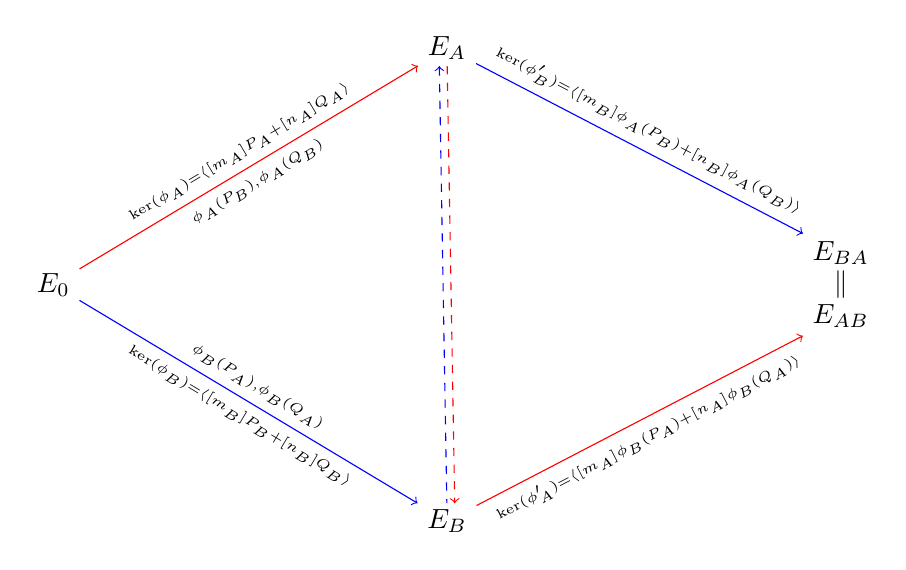
\begin{tikzpicture}
\node (1) at (-5cm,0cm){$E_0$};

\node (2) at (0cm,3cm){$E_A$};
\draw [color = red, ->] (1) -- (2);
\path (1) -- (2) node [above,sloped,pos=0.5]{$\scriptscriptstyle\ker(\phi_A)=\cyc{[m_A]P_A+[n_A]Q_A}$};
\path (1) -- (2) node [below,sloped,pos=0.5]{$\scriptscriptstyle\phi_A(P_B),\phi_A(Q_B)$};

\node (3) at (0cm,-3cm){$E_B$};
\draw [color = blue, ->] (1) -- (3);
\path (1) -- (3) node [below,sloped,pos=0.5]{$\scriptscriptstyle\ker(\phi_B)=\cyc{[m_B]P_B+[n_B]Q_B}$};
\path (1) -- (3) node [above,sloped,pos=0.5]{$\scriptscriptstyle\phi_B(P_A),\phi_B(Q_A)$};

\node (2a) at (0cm,2.9cm){};
\node (2b) at (-.1cm,2.9cm){};

\node (3a) at (.1cm,-2.9cm){};
\node (3b) at (0cm,-2.9cm){};

\draw [color = red, dashed, ->] (2a) -- (3a);
\draw [color = blue, dashed, <-] (2b) -- (3b);

\node (4) at (5cm,-.4cm){$E_{AB}$};
\draw [color = red, ->] (3) -- (4);
\path (3) -- (4) node [below,sloped,pos=0.5]{$\scriptscriptstyle\ker(\phi_A')=\cyc{[m_A]\phi_B(P_A)+[n_A]\phi_B(Q_A)}$};

\node (5) at (5cm,.4cm){$E_{BA}$};
\draw [color = blue, ->] (2) -- (5);
\path (2) -- (5) node [above,sloped,pos=0.5]{$\scriptscriptstyle\ker(\phi_B')=\cyc{[m_B]\phi_A(P_B)+[n_B]\phi_A(Q_B)}$};

\node (6) at (5cm,0cm){$\|$};

\end{tikzpicture}
\end{center}




\end{frame}

\begin{frame}
\frametitle{Security assumption}

\begin{problem}[Supersingular Isogeny (SSI) problem] Let $\phi_A
  \colon E_0 \to E_A$ be an isogeny whose kernel is
  $\cyc{[m_A]P_A+[n_A]Q_A}$, where $m_A$ and $n_A$ are chosen at
  random from $\Z/\ell_A^{e_A}\Z$ and not both divisible by $\ell_A$.
  Given $E_A$ and the values $\phi_A(P_B)$, $\phi_A(Q_B)$, find a
  generator $R_A$ of $\cyc{[m_A]P_A+[n_A]Q_A}$.
\end{problem}

\ 

The (Childs et al., 2010) attack against (Stolbunov, 2010) does not
work on supersingular curves, since there is no abelian class group.

\end{frame}

\begin{frame}
\frametitle{Attacks against the scheme}
Fastest known attack (given $E$ and $E_A$):
\begin{itemize}
\item Build a tree of degree $\ell_A$-isogenies of depth $e_A/2$
  starting from $E$
\item Build a tree of degree $\ell_A$-isogenies of depth $e_A/2$
  starting from $E_A$
\item Find a common vertex between the two trees 
\end{itemize}
Using claw-finding algorithms, one can solve this problem in:
\begin{itemize}
\item $O(p^{1/4})$ time on a classical computer
\item $O(p^{1/6})$ time on a quantum computer
\end{itemize}
Assuming that this is indeed the fastest possible attack, we need a
$768$-bit prime for $128$-bit security against quantum computers.
\end{frame}

\begin{frame}
\frametitle{Implementation}
To compute $\phi_A\colon E \to E/\<R_A\>$:
\begin{itemize}
\item Set $R_0 := [m_A]P_A + [n_A]Q_A$.
\item For $0\le i <e_A$, set
\begin{equation*}
  E_{i+1} = E_i/\<\ell_A^{e_A-i-1}R_i\>,\quad
  \phi_i : E_i \to E_{i+1},\quad
  R_{i+1} = \phi_i(R_i)
\end{equation*}
\item Then $\phi_i$ is a degree $\ell_A$ isogeny from $E_i$ to $E_{i+1}$.
\item We have
\begin{align*}
E_A &= E_{e_A} \\
\phi_A &=\phi_{e_A-1}\circ\cdots\circ\phi_0
\end{align*}
\end{itemize}
\end{frame}

\begin{frame}
\frametitle{Structure of the graph of isogenies}
\begin{center}
 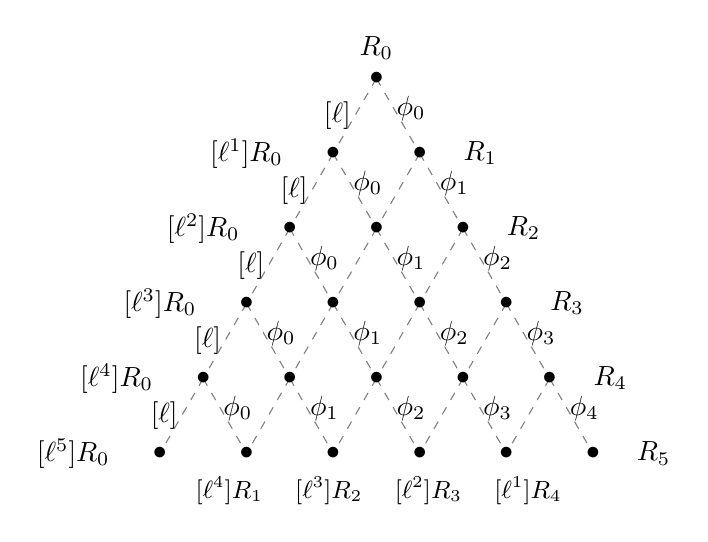
\begin{tikzpicture}[/triangle,scale=1.1]
    \def\n{5}
    \pgfmathtruncatemacro{\pn}{\n-1}
    

    \draw(-0.4,-0.2) node{$R_0$};

    \foreach \i in {1,...,\n} {
      \draw(\i,\i+0.7) node{$R_\i$};
    }
    \foreach \i in {1,...,\n} {
      \draw(\i,-1) node{$[\ell^\i]R_0$};
    }
    \foreach \i in {0,...,\pn} {
      \pgfmathtruncatemacro{\ii}{\pn-\i}
      \foreach \j in {0,...,\ii} {
        \draw(\i+\j+0.4,\i+0.6) node{$\phi_\i$};
      }
    }
    \foreach \i in {0,...,\pn} {
      \draw(\i+0.5,-0.2) node{$[\ell]$};
    }

    \foreach \i in {1,...,\pn} {
      \pgfmathtruncatemacro{\ii}{\n-\i}
      \draw(\n+0.5,1.15*\i-0.1) node{{\small $[\ell^\ii]R_\i$}};
    }

    \foreach \i in {0,...,\pn} {
      \foreach \j in {0,...,\i} {
        \draw[gray,dashed]  (\i,\j) -- (\i+1,\j+1);
        \draw[gray,dashed]  (\i,\j) -- (\i+1,\j);
      }
    }

    \dottriangle[$\bullet$]{\n}
  \end{tikzpicture}
\end{center}
For each $i$, one needs to compute $[\ell^{e-i}]R_i$ in order to
compute $\phi_i$.
\end{frame}

\begin{frame}
  \frametitle{Computational strategies}
\begin{figure}
\centering
  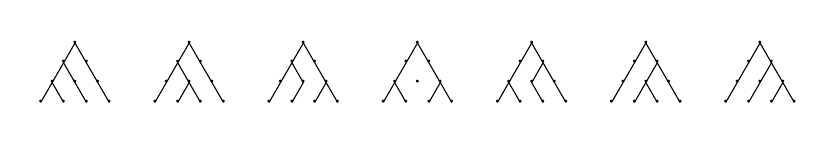
\begin{tikzpicture}[/triangle,scale=0.29]
    \def\n{3}
    \newlength{\shift}
    \setlength{\shift}{5cm}

    \foreach \k in {0,...,6} {
      \begin{scope}[xshift=\k\shift]
        \dottriangle[$\cdot$]{\n}
        \foreach \i in {1,...,\n} {
          \draw(\i-1,0) -- (\i,0);
        }
        \foreach \i in {1,...,\n} {
          \draw(\i-1,\i-1) -- (\i,\i);
        }
      \end{scope}
    }

    \begin{scope}
      \draw (1,0)--(2,1) (2,1)--(3,2) (2,0)--(3,1);
    \end{scope}

    \begin{scope}[xshift=\shift]
      \draw (1,0)--(2,1) (2,1)--(3,1) (2,1)--(3,2);
    \end{scope}

    \begin{scope}[xshift=2\shift]
      \draw (1,0)--(2,1) (2,1)--(3,1) (2,2)--(3,2);
    \end{scope}

    \begin{scope}[xshift=3\shift]
      \draw (2,0)--(3,1) (2,2)--(3,2);
    \end{scope}

    \begin{scope}[xshift=4\shift]
      \draw (1,1)--(2,1) (2,1)--(3,2) (2,0)--(3,1);
    \end{scope}

    \begin{scope}[xshift=5\shift]
      \draw (1,1)--(2,1) (2,1)--(3,2) (2,1)--(3,1);
    \end{scope}

    \begin{scope}[xshift=6\shift]
      \draw (1,1)--(2,1) (2,1)--(3,1) (2,2)--(3,2);
    \end{scope}
  \end{tikzpicture}
  \caption{The seven well formed strategies for $e=4$.}
\end{figure}

\begin{itemize}
\item We call the left-most strategy the \emph{isogeny-based} strategy.
\item We call the right-most strategy the \emph{multiplication-based}
  strategy.
\item In the published article, we only considered the above two
  strategies, but we subsequently realized that the intermediate
  strategies are asymptotically faster.
\end{itemize}
\end{frame}

\begin{frame}
\frametitle{Optimal strategy}
\begin{figure}[t]
  \centering
  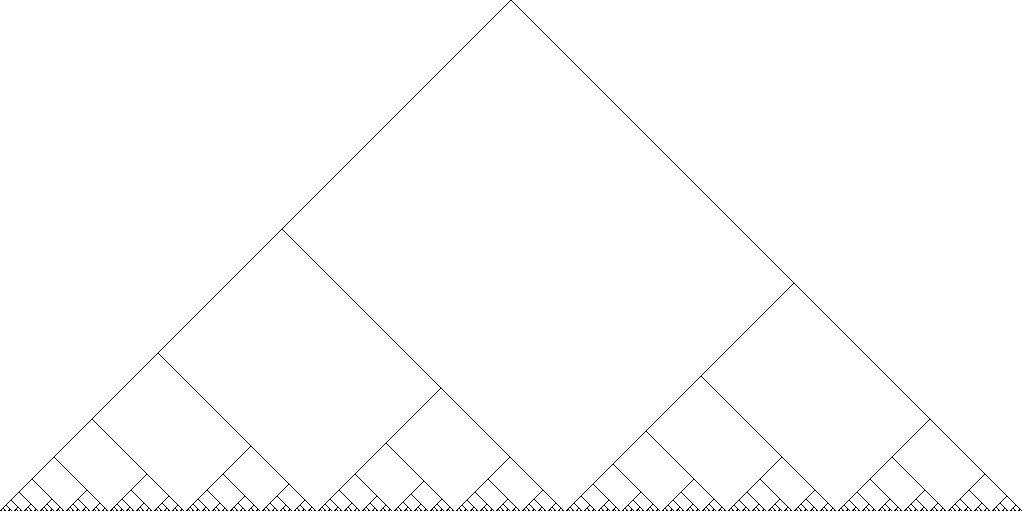
\includegraphics[width=0.8\textwidth]{../optimal.png}
  \caption{Optimal strategy for $e=512$, $\ell=2$.}
  \label{fig:optimal}
\end{figure}

The tree is asymmetric because the left branches (scalar
multiplication by $2$) are more expensive than the right branches
(evaluating degree $2$ isogenies).
\end{frame}

\begin{frame}
\frametitle{Asymptotic cost}
If $\alpha$ is the cost of one
multiplication (one left branch) and $\beta$ is the cost of one
isogeny (one right branch), the asymptotic cost of the optimal
strategy grows as
\[
    O(e \log_r e)
\]
where $e$ is the tree depth and $r$ is the solution to the equation
\[
   1 = r^{-\alpha} + r^{-\beta}
\]
The values of $r$ are related to generalized Fibonacci numbers (if
$\alpha=2,\beta=1$ then $r$ is the golden ratio).
\end{frame}

\begin{frame}
\frametitle{Timings}
{\small
  \begin{tabular}{c | c | r | r | r | r}
     & & \multicolumn{2}{c|}{Alice ($\ell=2$)} & \multicolumn{2}{|c}{Bob ($\ell=3$)}\\
    bit size & prime & round 1 & round 2 & round 1 & round 2\\
    \hline
    512 & $2^{258}3^{161}186-1$ &  63 ms &  56 ms &  83 ms &  69 ms \\
    \hline
    768 & $2^{386}3^{242}2-1$ & 128 ms & 114 ms &  163 ms &  135 ms \\
    \hline
    1024 & $2^{514}3^{323}353-1$ & 222 ms & 196 ms & 279 ms & 230 ms\\
  \end{tabular}
}

\ 

Operation counts for $\ell=2$ in $\F_{p^2}$ operations:
\begin{center}
\begin{tabular}{|c|c|} \hline
512 bits & 5072M + 2984S \\ \hline
768 bits & 8168M + 4788S \\ \hline
1024 bits & 11415M + 6701S \\ \hline
\end{tabular}
\end{center}

\ 

\ 

Source code available at \url{http://www.prism.uvsq.fr/~dfl/}
\end{frame}

\begin{frame}
\frametitle{References}
\small
\begin{itemize}
\item D. Charles, E. Goren, and K. Lauter. Cryptographic hash functions
from expander graphs. J. Cryptol. 2009, pp. 93--113.
\item J. Couveignes, Hard Homogeneous Spaces, eprint:2006/291.
\item A. Childs, D. Jao and V. Soukharev, Constructing elliptic curve
  isogenies in quantum subexponential time, arXiv:1012.4019.
\item A. Rostovtsev and A. Stolbunov, Public-key cryptosystem based on
  isogenies, eprint:2006/145.
\item A. Stolbunov, Constructing public-key cryptographic schemes
  based on class group action on a set of isogenous elliptic curves,
  Adv. Math. Comm. 4 (2) (2010), pp. 215--235.
\item J. V\'elu, Isog\'enies entre courbes elliptiques,
  C. R. Acad. Sci. Paris S\'er. A-B \textbf{273} (1971),
  pp. A238--A241.
\item W. Waterhouse, Abelian varities over finite fields,
  Ann. scient. \'Ec. Norm. Sup., series 4 vol. 2 (4) (1969),
  pp. 521--560.
\end{itemize}
\end{frame}

\end{document}

